\frame{
\frametitle{Simulations}
\begin{textblock*}{90mm}[0,0](-5mm,-2mm)
	\textcolor{myred}{\textbf{Resolved particle approaches}}
\end{textblock*}

\begin{textblock*}{125mm}[0,0](-8mm,2mm)
%\small{\textbf{Fluid equations:}}
%	\scriptsize{
%	\begin{eqnarray*}
%		\frac{\partial {u_i}}{\partial {t}}+\frac{\partial {u_ju_i}}{\partial {x_j}}
%		&=&
%		-\frac{1}{\rho}\frac{\partial {p}}{\partial {x_i}} 
%		+\nu\frac{\partial^2 {u_i}}{\partial {x_j}\partial {x_j}} +{f_i} -{f_i^{(p)}}
%		+{F_{i}}^0,\\
%		\frac{\partial u_i}{\partial x_i}&=&0.
%		\label{navier-stokes}
%	\end{eqnarray*}
%}
{\small
\begin{itemize}
	\item Finite size particles
	\item Key advantages: \vspace{-6pt}
	\begin{itemize}
		\item exact surface stress
		\item exact drag
		\item no undisturbed velocity needed
	\end{itemize}
	\item Key limitations:\vspace{-6pt}
	\begin{itemize}
	\item computational cost	
	\item fewer particles
	\item lower $R_{\lambda}$
\end{itemize}
\end{itemize}
}
\vspace{4pt}
\only<1>
\small{\textbf{A wide range of methods:}}
\begin{itemize}
	\item Immersed Boundary Method \vspace{-6pt}
	\item Force Coupling Method \vspace{-6pt}
	\item Lattice Boltzmann\vspace{-6pt}
	\item Basilisk\vspace{-6pt}
	\item Physalis\vspace{-6pt}
	\item \ldots
\end{itemize}
\vspace{-2pt}
{\footnotesize See review by Maxey, ARFM, 2017}
%
\end{textblock*}
%
\begin{textblock*}{80mm}[0,0](58mm,-4mm)
	\flushleft
	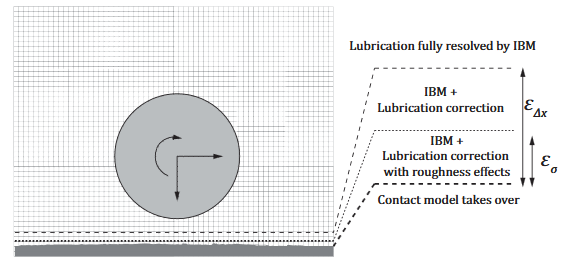
\includegraphics[clip,trim=0 0 0 30,height = 23mm]{IBM.png}\\
	\vspace{-7pt}
	{\hspace{10pt} {\tiny IBM: Costa et al, PRE, 2015}}	
\end{textblock*}
%
\begin{textblock*}{80mm}[0,0](65mm,28mm)
	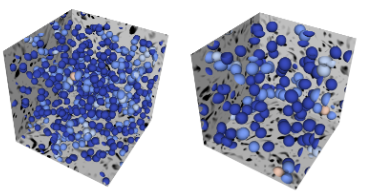
\includegraphics[height = 24mm]{basilisk.png}\\
	\vspace{-12pt}
	{\flushright {\tiny Basilisk: Boniou et al, JFM, 2025}}	
\end{textblock*}
%
\begin{textblock*}{50mm}[0,0](55mm,60mm)
	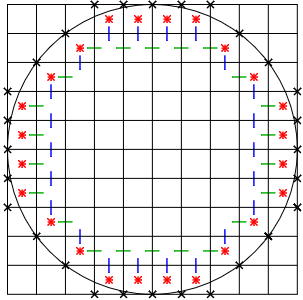
\includegraphics[height = 21mm]{physalis_1.png}
	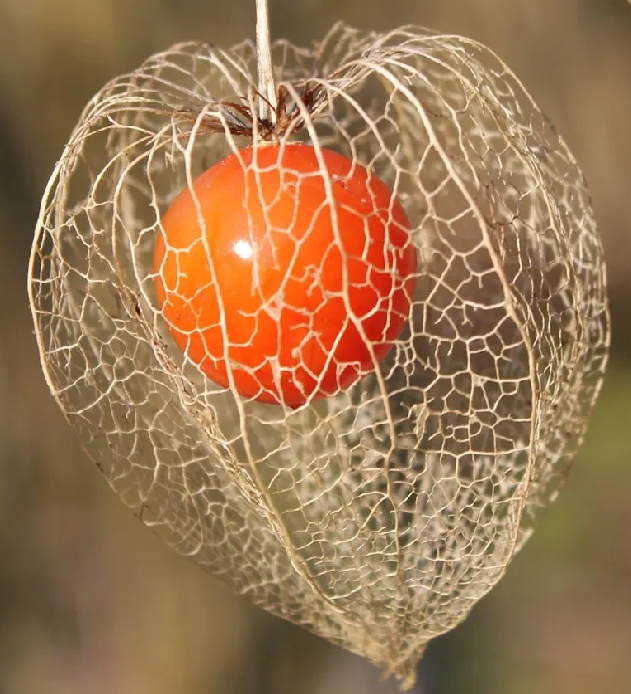
\includegraphics[height = 21mm]{physalis_2.png}\\
	\vspace{-6pt}
	{\tiny Physalis: Naso \& Prosperetti, NJP, 2010}	
\end{textblock*}

}